\section{Heavy quarks in cosmic plasma} \label{Bottom}

The primordial quark-gluon plasma (QGP) refers to the state of matter that existed in the early Universe, specifically for time $t\approx10\, \mathrm{\mu s}$ after the Big Bang. At that time the Universe was controlled by the strongly interacting particles: quarks and gluons. In this chapter, I study the heavy bottom and charm flavor quarks near to the QGP hadronization temperature $0.3\,\mathrm{GeV}>T>0.15\,\mathrm{GeV}$ and examine the relaxation time for the production and decay of bottom/charm quarks then show that the bottom quark nonequliibrium occur near to QGP –hadronization and create the arrow in time in the early Universe.

%~~~~~~~~~~~~~~~~~~~~~~~~~~~~~~~~~~~~~~~~~~~~~~~~~

\subsection{Overview of heavy quarks in primordial QGP}
%In this section we will focus on the following:
%\begin{itemize}
%    \item Review of primordial Quark-Gluon Plasma
%    \item Briefly remark the top quark
%\end{itemize}




In the QGP epoch, up and down $(u,d)$ (anti)quarks are effectively massless and remain in equilibrium via quark-gluon fusion. Strange $(s)$ (anti)quarks are in equilibrium via weak, electromagnetic, and strong interactions until $T\approx13$ MeV~\cite{Yang:2021bko}. The massive top $(t)$ (anti)quarks decay via the channel $t\to W+b$, with $\Gamma_t=1.4\pm0.2$\;GeV \cite{ParticleDataGroup:2018ovx} which implies that no bound state of top quarks have time to form. Given the large value of $\Gamma_t$ we realize that top quarks in hot QGP can be produced by the $ W+b\to t$ fusion process -- given the strength of this process there is no freeze-out of top quarks until $W$ itself freezes out. To address the top quarks in QGP, a dynamic theory for $W$ abundance is needed, a topic we will consider in the future. Finally, the bottom $(b)$ and charm $(c)$ quarks can be produced from strong interactions via quark-gluon pair fusion processes and disappear via weak interaction decays, and their abundance depends on the competition between the strong fusion and weak decay reaction rates.

The properties of QGP can be studied by experimental observations from high-energy heavy-ion collision experiments, such as  the Relativistic Heavy Ion Collider (RHIC) and the Large Hadron Collider (LHC). However, the conditions in the early Universe and those created in relativistic collisions are different. For example, the primordial QGP survives for about $10\mu$s in the cosmological Big Bang. On the other hand, the QGP formed in micro-bangs resulting from ultra-relativistic nuclear collisions has a lifespan of around  $10^{-23}$ s~\cite{Rafelski:2001hp}. Due to the considerably slower expansion rate of the Universe compared to quark production reactions and decays, in practicality, quark remained in equilibrium, and the quark fugacity is $\Upsilon=1$ during the QGP epoch.


However near the hadronization temperature, the heavy quarks abundance and deviations from chemical equilibrium have not yet been studied in great detail. In following we will focus on bottom and charm quarks. We will show that the bottom quarks can deviate from chemical equilibrium $\Upsilon\neq1$ by breaking the detailed balance between production and decay reactions of the quarks.


%~~~~~~~~~~~~~~~~~~~~~~~~~~~~~~~~~~~~~~~~~~~~~~~~~

\subsection{Bottom and Charm quark near QGP hadronization}
%In this section we will focus on the following:
%\begin{itemize}
%    \item Bottom/charm quarks production and decay in primordial QGP 
%    \item Dynamic equation for  bottom abundance (Stationary and non-stationary fugacity)
%    \item Nonstationary departure from detailed balance
%\end{itemize}
In the following we consider the temperature near QGP hadronization $0.3\,\mathrm{GeV}>T>0.15\,\mathrm{GeV}$, and study the bottom and charm abundance by examining the relevant reaction rates of their production and decay.
In thermal equilibrium the number density of light quarks can be evaluated in the massless limit, and we have
\begin{align}\label{FermiN}
n_q=\frac{g_{q}}{2\pi^2}\,T^3 F(\Upsilon_q)\;, \quad F=\int_0^\infty \frac{x^2dx}{1+\Upsilon_q^{-1}e^x}\;,
\end{align}
where $\Upsilon_q$ is the quark fugacity. We have $ F(\Upsilon_q=1)=3\,\zeta(3)/2$ with the Riemann zeta function $\zeta(3)\approx1.202$.
The thermal equilibrium number density of heavy quarks with mass $m\gg T$ can be well described by the Boltzmann expansion of the Fermi distribution function, giving
\begin{align}\label{BoltzN}
n_{q}\!=\!\frac{g_{q}T^3}{2\pi^2}\sum_{n=1}^{\infty}\frac{(-1)^{n+1}\Upsilon_q^n}{n^4}\left(\frac{n\,m_{q}}{T}\right)^{\!2}\!K_2\left(\frac{n\,m_{q}}{T}\right),
\end{align} 
where $K_2$ is the modified Bessel functions of integer order $2$. In the case of interest, when $m\gg T$, it suffices to consider the Boltzmann limit and  keep the first term $n=1$ in the expansion. The first term  $n=1$ also suffices for both charmed $c$-quarks and bottom $b$-quarks, giving
\begin{align}
&n_{b,c}={\Upsilon_{b,c}\,}n^{th}_{b,c},\qquad n^{th}_{b,c}=\frac{g_{b,c}}{2\pi^2}\,T^3\left(\frac{m_{b,c}}{T}\right)^2\,K_2(m_{b,c}/T).
\end{align}
However, for strange $s$ quarks, several terms are needed. 
%~~~~~~~Figure1~~~~~~~~~~~~~~~~~~~~~~~~~~~~~~~~~~~~~~~~~~~~~~~~~~~~~~~~~~~~~~~~~~~~~~~~~~~~~~~~~
\begin{figure}[t]
\begin{center}
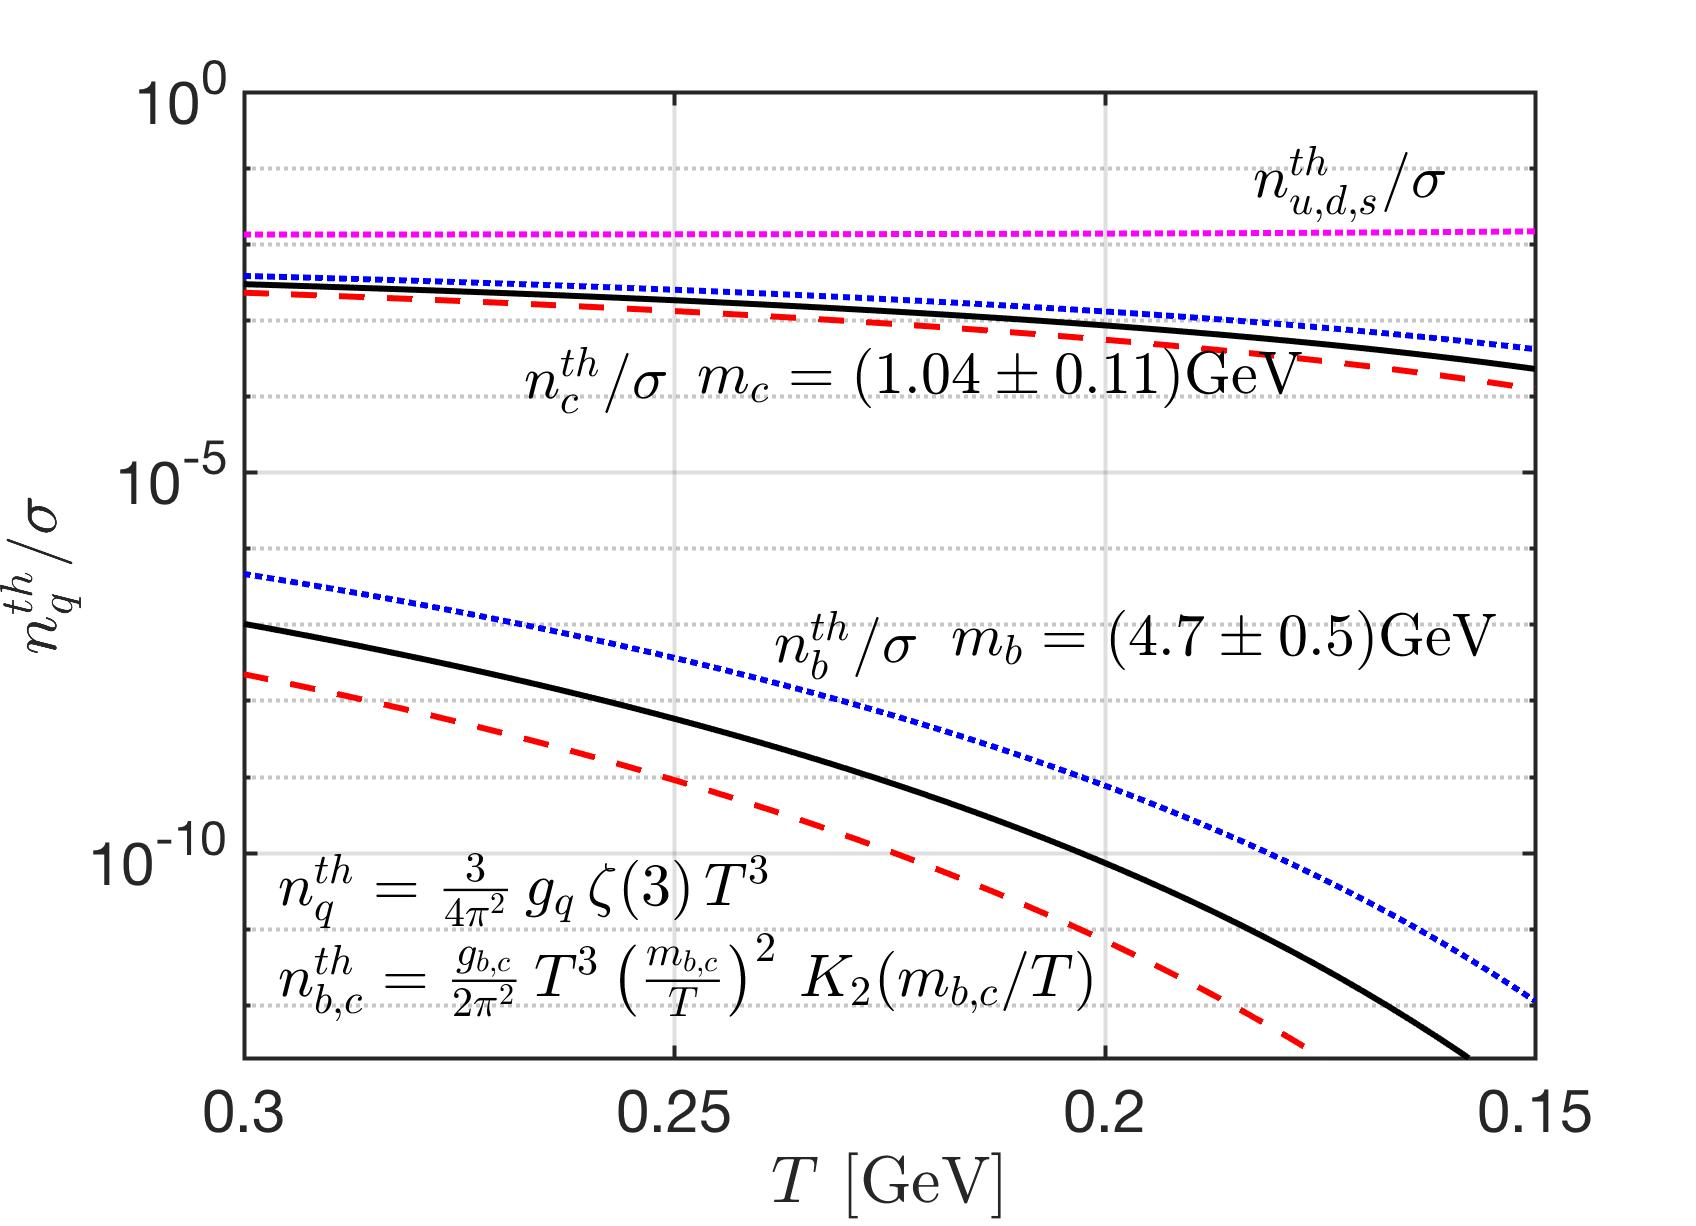
\includegraphics[width=0.9\textwidth]{./plots/bcQuarkDensity_new}
\caption{
The quark number density normalized by entropy density, as a function of temperature in the early Universe with $\Upsilon=1$. The $b$-quark mass parameters shown are $m_b=4.2\,\mathrm{GeV}$ (blue) dotted line, $m_b=4.7\,\mathrm{GeV}$ (black) solid line, and $m_b=5.2\,\mathrm{GeV}$ (red) dashed line. For  $c$-quark  $m_c=0.93\,\mathrm{GeV}$  (blue) dotted line, $m_c=1.04\,\mathrm{GeV}$ (black) solid line, and $m_c=1.15\,\mathrm{GeV}$ (red) dashed line. Adapted from thesis of C.T.Yang \cite{Yang:2024ret}.}
\label{number_entropy_b002}
\end{center}
\end{figure}
%~~~~~~~~~~~~~~~~~~~~~~~~~~~~~~~~~~~~~~~~~~~~~~~~~~~~~~~~~~~~~~~~~~~~~~~~~~~~~~~~~~~~~~~~~~~~~


In Fig.~\ref{number_entropy_b002} we show the equilibrium ($\Upsilon=1$) number density per entropy density  ratio as a function of temperature $T$ of quarks. The entropy density is given by Eq.~(\ref{entropy}) and only light particles contribute to the entropy density; thus the result we consider is independent of actual abundance of $c$, $b$ and other heavy particles. We evaluated the density-per-entropy ratio for  $m_b=4.2,\;4.7,\;5.2$\,GeV and $m_c=1.04\pm0.11$\,GeV. The $m_b\simeq 5.2\,\mathrm{GeV}$ is  a typical potential model mass used in modeling bound states of bottom, and $m_b=4.2,\,4.7\,\mathrm{GeV}$ is the current quark mass at low and high energy scales. In Fig.~\ref{number_entropy_b002} we see that the charm abundance in the domain of interest $0.3\,\mathrm{GeV}>T>0.15\,\mathrm{GeV}$ is about $10^4\sim\!\!10^{9}$ times greater than the bottom quarks. This implies that the small $b$,$\bar b$ quark abundance is embedded in a large background comprising all lighter $u,d,s,c$ quarks and antiquarks, as well as gluons $g$.

\subsection{Reaction rate for quarks production and decay}
In primordial QGP, the bottom and charm quarks can be produced from strong interactions via quark-gluon pair fusion processes and disappear via weak interaction decays. For production, we have the following processes
\begin{align}
 q+\bar{q}&\longrightarrow b+\bar b,\qquad q+\bar{q}\longrightarrow c+\bar c,\\
 g+g&\longrightarrow b+\bar b,\qquad g+g\longrightarrow c+\bar c,
\end{align}
for bottom and charm we have
\begin{align}
 &b\longrightarrow c+l+\overline{\nu_l}, \qquad b\longrightarrow c+q+\bar{q},\\
&c\longrightarrow s+l+\overline{\nu_l},\qquad c\longrightarrow s+q+\bar{q},
\end{align}
for their decay. In following we will calculate the production rate and decay rate for bottom and charm quarks and compare to the Universe expansion rate. We will show that in the epoch of interest to us the characteristic Universe expansion time $1/H$ is much longer than the lifespan and production time of the bottom/charm quark. In this case, the dilution of bottom/charm quark due to the Universe expansion is slow compare to the the strong interaction production, and the weak interaction decay of the bottom/charm. 
 



%~~~~~~~~~~~~~~~~~~~~~~~~~~~~~~~~~~~~~~~~~~~~~~~~~~~~~~~~~~

\subsubsection{Quark production rate via strong interaction}
For the quark-gluon pair fusion processes
%\begin{align}
% q+q&\longrightarrow b+\bar b,\qquad q+q\longrightarrow c+\bar c,\\
% g+g&\longrightarrow b+\bar b,\qquad g+g\longrightarrow c+\bar c,
%\end{align}
the evaluation of the lowest-order Feynman diagrams yields the cross sections~\cite{Letessier:2002ony}:
\begin{align}
&\sigma_{q\bar{q}\rightarrow b\bar{b},c\bar{c}}=\frac{8\pi\alpha_s^2}{27s}\left(1+\frac{2m_{b,c}^2}{s}\right)w(s),\,\qquad w(s)=\sqrt{1-{4m^2_{b,c}}/{s}},\\
&\sigma_{gg\rightarrow b\bar{b},c\bar{c}}=\!\frac{\pi\alpha_s^2}{3s}\bigg[\left(1\!+\!\frac{4m^2_{b,c}}{s}\!+\!\frac{m^4_{b,c}}{s^2}\right)\ln{\left(\frac{1+w(s)}{1-w(s)}\right)}\!-\!\left(\frac{7}{4}\!+\!\frac{31m^2_{b,c}}{4s}\right)w(s)\bigg],
\end{align} 
where $m_{b,c}$ represents the mass of bottom or charm quark, $s$ is the Mandelstam variable, and $\alpha_s$ is the QCD coupling constant. Considering the perturbation expansion of the coupling constant $\alpha_s$ for the two-loop approximation~\cite{Letessier:2002ony}, we have:
\begin{align}
\alpha_s(\mu^2)=\frac{4\pi}{\beta_0\ln({\mu^2/\Lambda^2})}\bigg[1-\frac{\beta_1}{\beta_0}\frac{\ln(\ln{(\mu^2/\Lambda^2)})}{\ln(\mu^2/\Lambda^2)}\bigg],
\end{align}
where $\mu$ is the renormalization energy scale and $\Lambda^2$ is a parameter that determines the strength of the interaction at a given energy scale in QCD. The energy scale we consider is based on required gluon/quark collisions above $b\bar b$ energy threshold, so we have $\mu=2m_b+T$. For the energy scale $\mu>2m_b$ we have $\Lambda=180\sim230$ MeV( $\Lambda\approx205$ MeV in our calculation), and the parameters $\beta_0=11-2n_f/3$, $\beta_1=102-38n_f/3$ with the number of active fermions $n_f=4$. 

In general the thermal reaction rate per unit time and volume $R$ can be written in terms of the scattering cross section as follows~\cite{Letessier:2002ony}:
\begin{align}
R\equiv\sum_i\int_{s_{th}}^\infty\!ds\,\frac{dR_i}{ds}=\sum_i\int_{s_{th}}^\infty\!ds\,\sigma_i(s)\,P_i(s),
\end{align}
where $\sigma_i(s)$ is the cross section of the reaction channel $i$, and $P_i(s)$ is the number of collisions per unit time and volume. Considering the quantum nature of the colliding particles (i.e., Fermi and Bose distribution) with the massless limit and chemical equilibrium condition ($\Upsilon=1$), we obtain~\cite{Letessier:2002ony}
\begin{align}
&P_i(s)=\frac{g_1g_2}{32\pi^4}\,\frac{T}{1+I_{12}}\frac{\lambda_2}{\sqrt{s}}\!\sum_{l,n=1}^{\infty}\!(\pm)^{l+n}\frac{K_1(\sqrt{lns}/T)}{\sqrt{ln}},\\
&\lambda_2\equiv\left[s-\left(m_1+m_2\right)^2\right]\,\left[s-\left(m_1-m_2\right)^2\right],
\end{align}
where $+$ is for boson and $-$ is for fermions, and the factor $1/(1+I_{12})$ is introduced to avoid double counting of indistinguishable pairs of particles. $I_{12}=1$ for identical pair of particles, otherwise $I_{12}=0$. Hence the total thermal reaction rate per volume for bottom quark production can be written as
\begin{align}
\label{Bquark_Source}
R^{\mathrm{Source}}_{b,c}=\int^\infty_{s_{th}}ds\,\bigg[\sigma_{q\bar{q}\rightarrow b\bar{b},c\bar{c}}\,P_q+\sigma_{gg\rightarrow b\bar{b},c\bar{c}}\,P_g\bigg]%=R_{q\bar{q}\rightarrow b\bar{b},c\bar{c}}+R_{gg\rightarrow b\bar{b},c\bar{c}}.
\end{align}
We introduce the bottom/charm quark relaxation time for the quark-gluon pair fusion as follows:
\begin{align}
\label{relaxation_time}
&{\tau_{b,c}^{\mathrm{Source}}}\equiv\frac{dn_{b,c}/d\Upsilon_{b,c}}{R^{\mathrm{Source}}_{b,c}}\;,\quad
\end{align}
where $dn_{b,c}/d\Upsilon_{b,c}=n^{th}_{b,c}$ in the Boltzmann approximation. The relaxation time is on the order of magnitude of time needed to reach chemical equilibrium. In Fig.~\ref{BCreaction_fig} we show the characteristic time for bottom/charm  quark strong interaction production in the domain of interest, $ 0.3\,\mathrm{GeV}>T> 0.15\,\mathrm{GeV}$. 

\subsubsection{Quark decay rate via weak interaction}
The bottom/charm quark decay via the weak interaction. 
%\begin{align}
% &b\longrightarrow c+l+\nu_l, \qquad %b\longrightarrow c+q+\bar{q},\\
%&c\longrightarrow s+l+\nu_l,\qquad c\longrightarrow s+q+\bar{q},
%\end{align}
The vacuum decay rate for $1\to2+3+4$ in vacuum can be evaluated via the weak interaction:
\begin{align}
\frac{1}{\tau_1}=&\frac{64G^2_F\,V^2_{12}\,V^2_{34}}{(4\pi)^3g_1}\,m^5_1\times\left[\frac{1}{2}{\left(1-\frac{m^2_2}{m^2_1}-\frac{m^2_3}{m^2_1}+\frac{m^2_4}{m^2_1}\right)}\mathcal{J}_1-\frac{2}{3}\mathcal{J}_2\right],
\end{align}
where the Fermi constant is $G_F=1.166\times10^{-5}\,\mathrm{GeV}^{-2}$, $V_{ij}$ is the element of the Cabibbo-Kobayashi-Maskawa (CKM) matrix~\cite{Czarnecki:2004cw} for quark channel and $V_{l\nu_l}=1$ for lepton channel. The functions $\mathcal{J}_1$ and $\mathcal{J}_2$ are given by
\begin{align}
&\mathcal{J}_1\!=\!\!\!\int_0^{(1-m^2_2/m^2_1)/2}\!\!\!\!\!\!\!\!dx\left(1\!-\!2x\!-\!\frac{m^2_2}{m_1^2}\right)^{\!\!2}\left[\frac{1}{(1-2x)^2}-1\right]\\
&\mathcal{J}_2\!=\!\!\!\int_0^{(1-m^2_2/m^2_1)/2}\!\!\!\!\!\!\!\!dx\left(1\!-\!2x\!-\!\frac{m^2_2}{m_1^2}\right)^{\!\!3}\left[\frac{1}{(1-2x)^3}-1\right]
\end{align}
The modification due to the heat bath(plasma) is small because the bottom and charm  mass $m_{b,c}\gg T$~\cite{Kuznetsova:2008jt}. In the temperature range we are interested in, the decay rate in the vacuum is a good approximation for our calculation. We show the lifespan for bottom/charm quark in Fig.~\ref{BCreaction_fig}. 

%there is no modification due to the phase space blocking because the bottom/charm mass is too heavier $m_{b,c}\gg T$~\cite{Kuznetsova:2008jt}. We did not include above either base enhancement nor fermi blocking factors since process of bottom decay involve energies beyond those available for $ 150< T< 300\,\mathrm{MeV}$.



%%%%%%%%%%%%%%%%%%%%%%%%%%%%%%%%%%%%%%%
\begin{figure} %[ht]
    \centering
    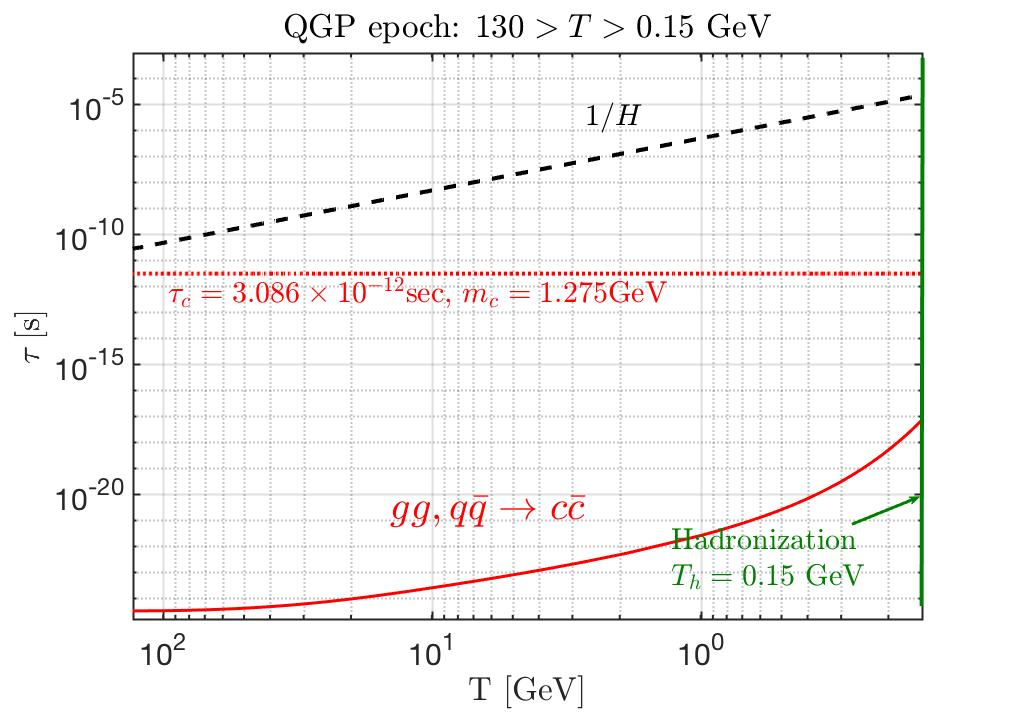
\includegraphics[width=0.85\textwidth]{./plots/CharmQuark_QGP.jpg}
    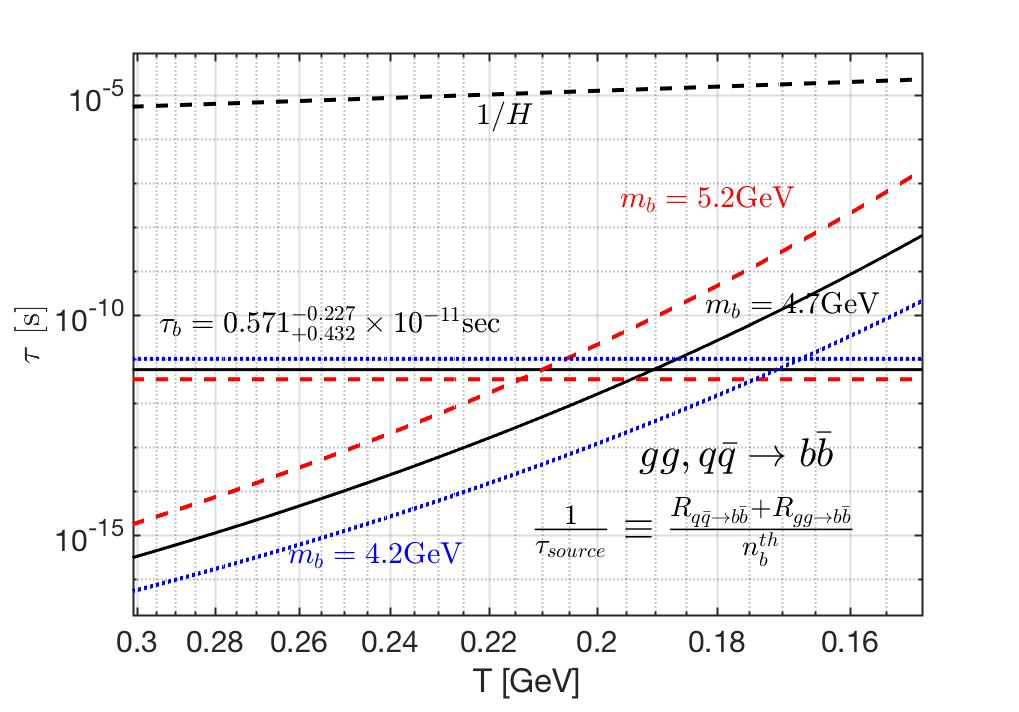
\includegraphics[width=0.85\textwidth]{./plots/BQuarkReactionTime_bottom.jpg}
    \caption{\cccite{universe9070309}, adapted from thesis of C.T.Yang \cite{Yang:2024ret}. Comparison of Hubble time $1/H$, quark lifespan $\tau_{q}$, and characteristic time for production via quark-gluon pair fusion for (top figure) charm and (bottom figure) bottom quarks as a function of temperature. Both figures end at approximately the hadronization temperature of $T_{H}\approx150$ MeV. Three different masses $m_{b}=4.2$ GeV (blue short dashes), $4.7$ GeV, (solid black), $5.2$ GeV (red long dashes) for bottom quarks are plotted to account for its decay width.}
\label{BCreaction_fig}
\end{figure}
%%%%%%%%%%%%%%%%%%%%%%%%%%%%%%%%%%%%%%%



%~~~~~~~~~~~~~~~~~~~~~~~~~~~~~~~~~~~~~~~~~~~~~~~~~~~~~~~~~~~~~~~~~~~~~~~~~~~~
\subsubsection{Hubble expansion rate}
In the early Universe, within a temperature range $130\, \mathrm{GeV}>T>0.15\,\mathrm{GeV}$,  we have the following particles:  photons, $8$ color charge gluons, $W^\pm$, $Z^0$, three generations of $3$ color charge quarks and leptons in the primordial QGP.  The Hubble parameter can be written in terms of particle energy density $\rho_i$
\begin{align}
H^2=\frac{8\pi G_N}{3}\left(\rho_\gamma+\rho_{\mathrm{lepton}}+\rho_{\mathrm{quark}}+\rho_{g,{W^\pm},{Z^0}}\right),
\end{align}
where $G_N$ is the Newtonian constant of gravitation. The effectively massless particles and radiation dominate the speed of expansion of the Universe. The characteristic Universe expansion time constant $1/H$ is seen in Fig.~\ref{BCreaction_fig}. In the epoch of interest to us $0.3\,\mathrm{GeV}>T>0.15\,\mathrm{GeV}$, the Hubble time $1/H\approx10^{-5}$ sec which is much longer than the lifespan and production time of the bottom and charm quarks. 
%~~~~~~~~~~~~~~~~~~~~~~~~~~~~~~~~~~~~~~~~~~~~~~~~~~~~~~~~~~~~~~~~~~~~~~~~~~~~~~~~~~~~~~~

\subsubsection{Rate Comparison: Strong fusion, Weak decay, and Hubble expansion}
In Fig.~\ref{BCreaction_fig} (top), we plot the relaxation time of the production/decay for charm quarks and Hubble time $1/H$ as a function of temperature. Throughout the entire duration of QGP, the Hubble time is larger than the lifespan and production times of the charm quark. %Therefore, the heavy charm quark remains in equilibrium as its processes occur faster than the expansion of the Universe. 
Additionally, the charm quark production time is faster than the decay. The faster quark-gluon pair fusion keeps the charm in chemical equilibrium up until hadronization. After hadronization, charm quarks form heavy mesons that decay into multi-particles quickly in plasma. The daughter particles from charm meson decay can interact and reequilibrate with
the plasma quickly. In this case the energy required for the inverse decay reaction to produce
charm meson is difficult to overcome and causing the charm quark to vanish from the inventory of particles via decay in the Universe.

In Fig.~\ref{BCreaction_fig} (bottom) we present the relaxation times for production and decay of the bottom quark with different masses as a function of temperature. It shows that both production and decay are faster than the Hubble time $1/H$ for the duration of QGP. However, unlike charm quarks, the relaxation time for bottom quark production intersects with bottom quark decay at different temperatures which depends on the mass of the bottom. The intersection implies that the bottom quark freeze-out from the primordial plasma before hadronization as the production process slows down at low temperatures and the subsequent weak interaction decay leads to a dilution of the bottom quark content within the QGP plasma. All of this occurs with rates faster than Hubble expansion and thus as the Universe expands, the system departs from a detailed chemical balance because of the competition between decay and production reactions in QGP. In this scenario, the dynamic equation on bottom abundance is required and causes the distribution to deviate from equilibrium with $\Upsilon\neq1$ in the temperature range below the crossing point but before the hadronization. 



\subsection{Bottom quark abundance nonequilibrium}

The competition between weak interaction decay and strong interaction production rates leads the dynamic bottom abundance in QGP. The dynamic equation for bottom quark abundance in QGP can be written as 
\begin{align}
\label{Bquark_eq}
\frac{1}{V}\frac{dN_b}{dt}=\big(\,1-\Upsilon^2_{b}\,\big)\,R^{\mathrm{Source}}_{b}-\Upsilon_b\,R^{\mathrm{Decay}}_{b}\;,
\end{align}
where $R^{\mathrm{Source}}_{b}$ and $R^{\mathrm{Decay}}_{b}$ are the thermal reaction rates per volume of production and decay of bottom quark, respectively. The bottom source rates are the gluon and quark fusion rates Eq.~(\ref{Bquark_Source}). The decay rate depends on whether the bottom quarks are freely present in the plasma or are bounded within mesons. We consider two extreme scenarios for the bottom quark population: 1.) all bottom flavor is free, and 2.) all bottom flavor is bounded into mesons in QGP. In Fig.~\ref{ReactionTime}  we show the characteristic interaction times relevant to the abundance of bottom quarks, as well as the Hubble time $1/H$ for the temperature range of interest, $0.3\,\mathrm{GeV}> T> 0.15\,\mathrm{GeV}$.

%~~~~~~~~~~~~~~~~~~~~~~~~~~~~~~~~~~~~~~~~~~~~~~~~~~~~~~~~~~~~~
\begin{figure}[ht]
\begin{center}
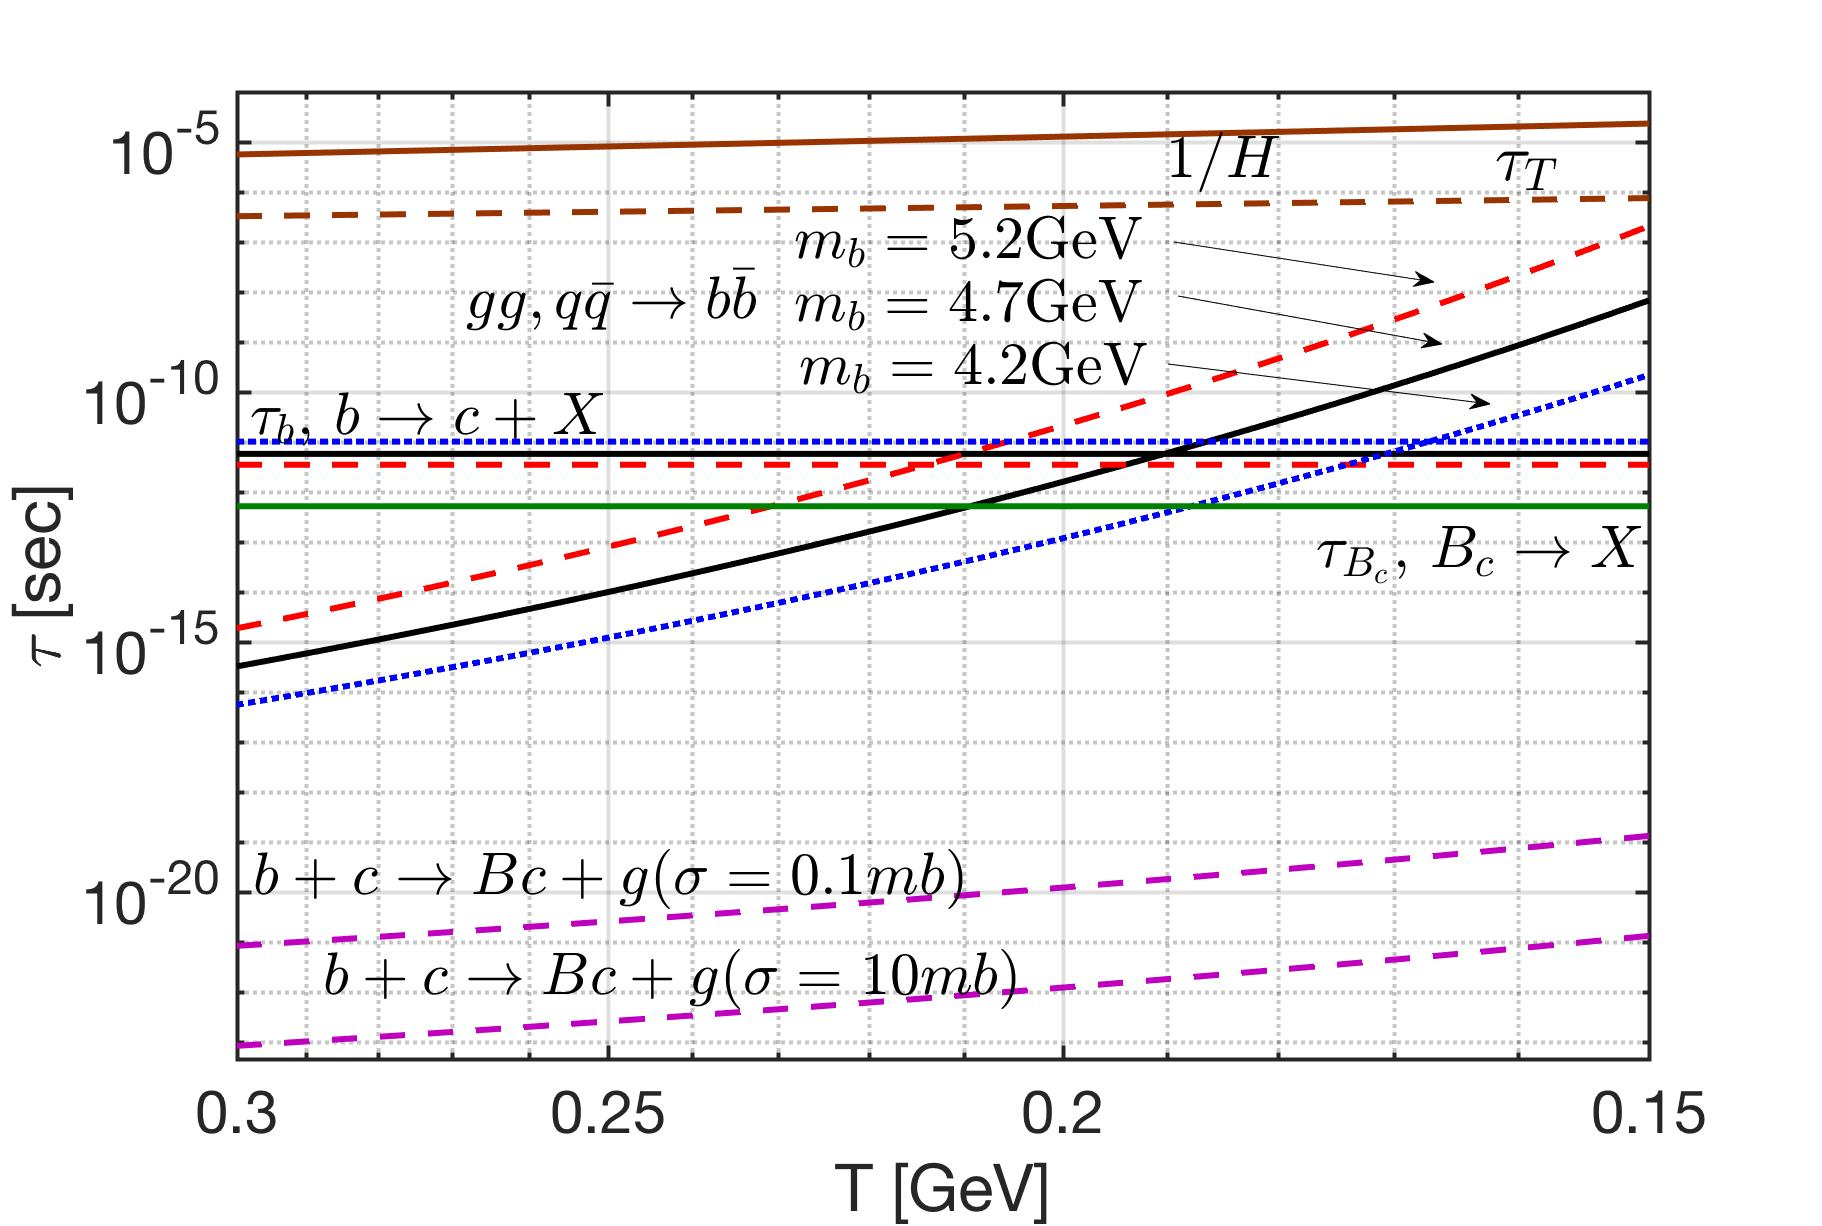
\includegraphics[width=0.85\textwidth]{./plots/BQuarkReactionTime003}
\caption{Production and decay characteristic times of bottom quark and the Hubble time $1/H$ within the temperature range of interest  $ 0.3\,\mathrm{GeV}>T> 0.15\,\mathrm{MeV}$. Near the top of figure  $1/H$ (brown solid line) and $\tau_T$ (brown dashed line); other horizontal lines are bottom-quark (in QGP) weak interaction lifetimes $\tau_b$ for the three different masses: $m_b=4.2\,\mathrm{GeV}$ (blue dotted line), $m_b=4.7\,\mathrm{GeV}$ (black solid  line), $m_b=5.2\,\mathrm{GeV}$ (red dashed line), and the vacuum lifespan $\tau_B$ of the  B$_c$ meson (green solid  line). The relaxation time for strong interaction bottom production $g+g, q+\bar q\rightarrow b+\bar{b}$ is shown with three different bottom masses and same type-color coding as weak interaction decay rate. At bottom of figure the in plasma formation process (dashed lines, purple) $b+c\rightarrow \mathrm{B}_c+g$ with cross section range $\sigma=0.1,10\,\mathrm{mb}$. Adapted from thesis of C.T.Yang \cite{Yang:2024ret}}
\label{ReactionTime}
\end{center}
\end{figure}
%~~~~~~~~~~~~~~~~~~~~~~~~~~~~~~~~~~~~~~~~~~~~~~~~~~~~~~~~~~~~~
Considering all bottom flavor is free in QGP, the bottom decay rate per volume is the bottom lifespan weighted with density of particles Eq.~(\ref{BoltzN})~~\cite{Kuznetsova:2008jt}. We have
\begin{align}\hspace{0.5cm}
R^{\mathrm{Decay}}_b=\frac{dn_b/d\Upsilon_b}{\tau_b},\,\,\,\,\, \tau_b\approx0.57\times10^{-11} \mathrm{sec}.
\end{align}
On the other hand, $b$,$\bar b$ quark abundance is embedded in a large background comprising all lighter quarks and antiquarks (see Fig.~\ref{number_entropy_b002}). After formation the heavy $b, \bar b$ quark can bind with any of the available lighter quarks, with the most likely outcome being a chain of reactions 
\begin{align}
&b+q\longrightarrow\mathrm{B}+g\;,\\
&\mathrm{B}+s\longrightarrow\mathrm{B}_s+q\;,\\
&\mathrm{B}_s+c\longrightarrow\mathrm{B}_c+s\;,
\end{align}
with each step providing a gain in binding energy and reduced speed due to the diminishing abundance of heavier quarks $s, c$. To capture the lower limit of the rate of $\mathrm{B}_c$ production we show in Fig.~\ref{ReactionTime} the expected formation rate by considering the direct process $b+\overline c\rightarrow \mathrm{B}_c+g$, considering the range of cross section $\sigma=0.1\sim10\,\mathrm{mb}$ ~\cite{Schroedter:2000ek}. The rapid formation rate of B$_c(b\bar c)$ states in primordial plasma is shown by purple dashed lines at bottom in Fig.~\ref{ReactionTime}, we have
\begin{align}
\tau (b+\overline c\rightarrow \mathrm{B}_c+g)\approx(10^{-16}\sim10^{-14})\times\frac{1}{H} \;.
\end{align}

Despite the low abundance of charm, the rate of $\mathrm{B}_c$ formation is relatively fast, and that of lighter flavored B-mesons is substantially higher. Note that as long as we have bottom quarks made in gluon/quark fusion bound practically immediately with any quarks $u, d, s$ into B-mesons, we can use the production rate of $b, \bar b$ pairs as the rate of B-meson formation in the primordial-QGP, which all decay with lifespan of pico-seconds. We believe that this process is fast enough to allow consideration of bottom decay from the B$_c(b\bar c)$, $\overline{\mathrm{B}}_c(\bar b c)$ states~\cite{Yang:2020nne}.  
 Based on the hypothesis that all bottom flavor is bound rapidly into $\mathrm{B}_c^\pm$ mesons, we have 
\begin{align}\label{Bc_source}
g+g, q+q \longleftrightarrow &b+\bar b\;[b(\bar{b})+\bar{c}(c)]\longrightarrow \mathrm{B}_c^\pm\longrightarrow\mathrm{anything}.
\end{align}
In this case, the decay rate per volume can be written as
\begin{align}\hspace{0.5cm}
 R^{\mathrm{Decay}}_b=\frac{dn_b/d\Upsilon_b}{\tau_{\mathrm{B}_c}},\,\,\,\,\, \tau_{\mathrm{B}_c}\approx0.51\times10^{-12} \mathrm{sec}.
 \end{align}



To investigate the nonequilibrium phenomena of bottom quarks, we aim to replace the variation of particle abundance seen on LHS in Eq.~(\ref{Bquark_eq}) by the time variation of abundance fugacity $\Upsilon$.
This substitution allows us to derive the dynamic equation for the fugacity parameter and enables us to study the fugacity as a function of time . Considering the expansion of the Universe we have
\begin{align}\label{number_dilution}
\frac{1}{V}\frac{dN_b}{dt}=\frac{dn_b}{d\Upsilon_b}\frac{d\Upsilon_b}{dt}+\frac{dn_b}{dT}\frac{dT}{dt}+3Hn_b,\;
\end{align}
where we use $d\ln(V)/dt=3H$ for the Universe expansion. Substituting Eq.~(\ref{number_dilution}) into Eq.~(\ref{Bquark_eq}) and dividing both sides of equation by $dn_b/{d\Upsilon_b}=n^{th}_b$, the fugacity equation becomes
\begin{align}
\frac{d\Upsilon_b}{dt}+&3H\Upsilon_b+\Upsilon_b\frac{dn^{th}_b/dT}{n^{th}_b}\frac{dT}{dt}=\left(1-\Upsilon_b^2\right)\frac{1}{\tau_{b}^{\mathrm{Source}}}-\Upsilon_b\frac{1}{\tau^{\mathrm{Decay}}_b}\;,
\end{align}
where relaxation time for bottom production is obtained using Eq.~(\ref{relaxation_time}). It is convenient to introduce the relaxation time $1/\tau_T$ as follows,
\begin{align}
\frac{1}{\tau_T}\equiv-\frac{dn^{th}_b/dT}{n^{th}_b}\frac{dT}{dt},
\end{align}
where we put '$-$' sign in the definition to have $\tau_T>0$. The relaxation time $\tau_T$ represents how the bottom density changes due to the Universe temperature cooling. In this case, the fugacity equation can be written as
\begin{align}\label{Fugacity_Eq0}
\frac{d\Upsilon_b}{dt}\!\!=&(1-\Upsilon_{b}^2)\frac{1}{\tau_{b}^{\mathrm{Source}}}
\!-\!\Upsilon_{b}\left(\frac{1}{\tau^{\mathrm{Decay}}_b}+3H\!-\!\frac{1}{\tau_T}\right).
\end{align}
In following sections we will solve the fugacity differential equation in two different scenarios: stationary and nonstationary Universe.

\subsubsection{First solution: stationary Universe}
In Fig.~\ref{BCreaction_fig} (bottom) we show that the relaxation time for both production and decay are faster than the Hubble time $1/H$ for the duration of QGP, which implies that $H,1/\tau_T\ll1/\tau_{b}^{\mathrm{Source}},1/\tau^{\mathrm{Decay}}_b$. In this scenario, we can solve the fugacity equation by considering the stationary Universe first, i.e., the Universe is not expanding and we have
\begin{align}\label{stationary}
H=0,\qquad1/\tau_T=0.
\end{align} 
In the stationary Universe at each given temperature we consider the dynamic equilibrium condition (detailed balance) between production and decay reactions that keep
\begin{align}
\frac{d\Upsilon_b}{dt}=0.
\end{align}
Neglecting the time dependence of the fugacity $d\Upsilon_b/dt$ and substituting the condition Eq.~(\ref{stationary}) into the fugacity equation Eq.~(\ref{Fugacity_Eq0}), then we can solve the quadratic equation to obtain the stationary fugacity as follows:
\begin{align}
\label{Fugacity_Sol}
\Upsilon_{\mathrm{st}}&=\sqrt{1+\left(\frac{\tau_{source}}{2\tau_{decay}}\right)^2}-\left(\frac{\tau_{source}}{2\tau_{decay}}\right).
\end{align}
%~~~~~~~Figure~~~~~~~~~~~~~~~~~~~~~~~~~~~~~~~~~~~~~~~~~~~~~~~~~~~~~~~~~~~~~~~~~~~~~~~~~~~~~~~~~
\begin{figure}[ht]
\begin{center}
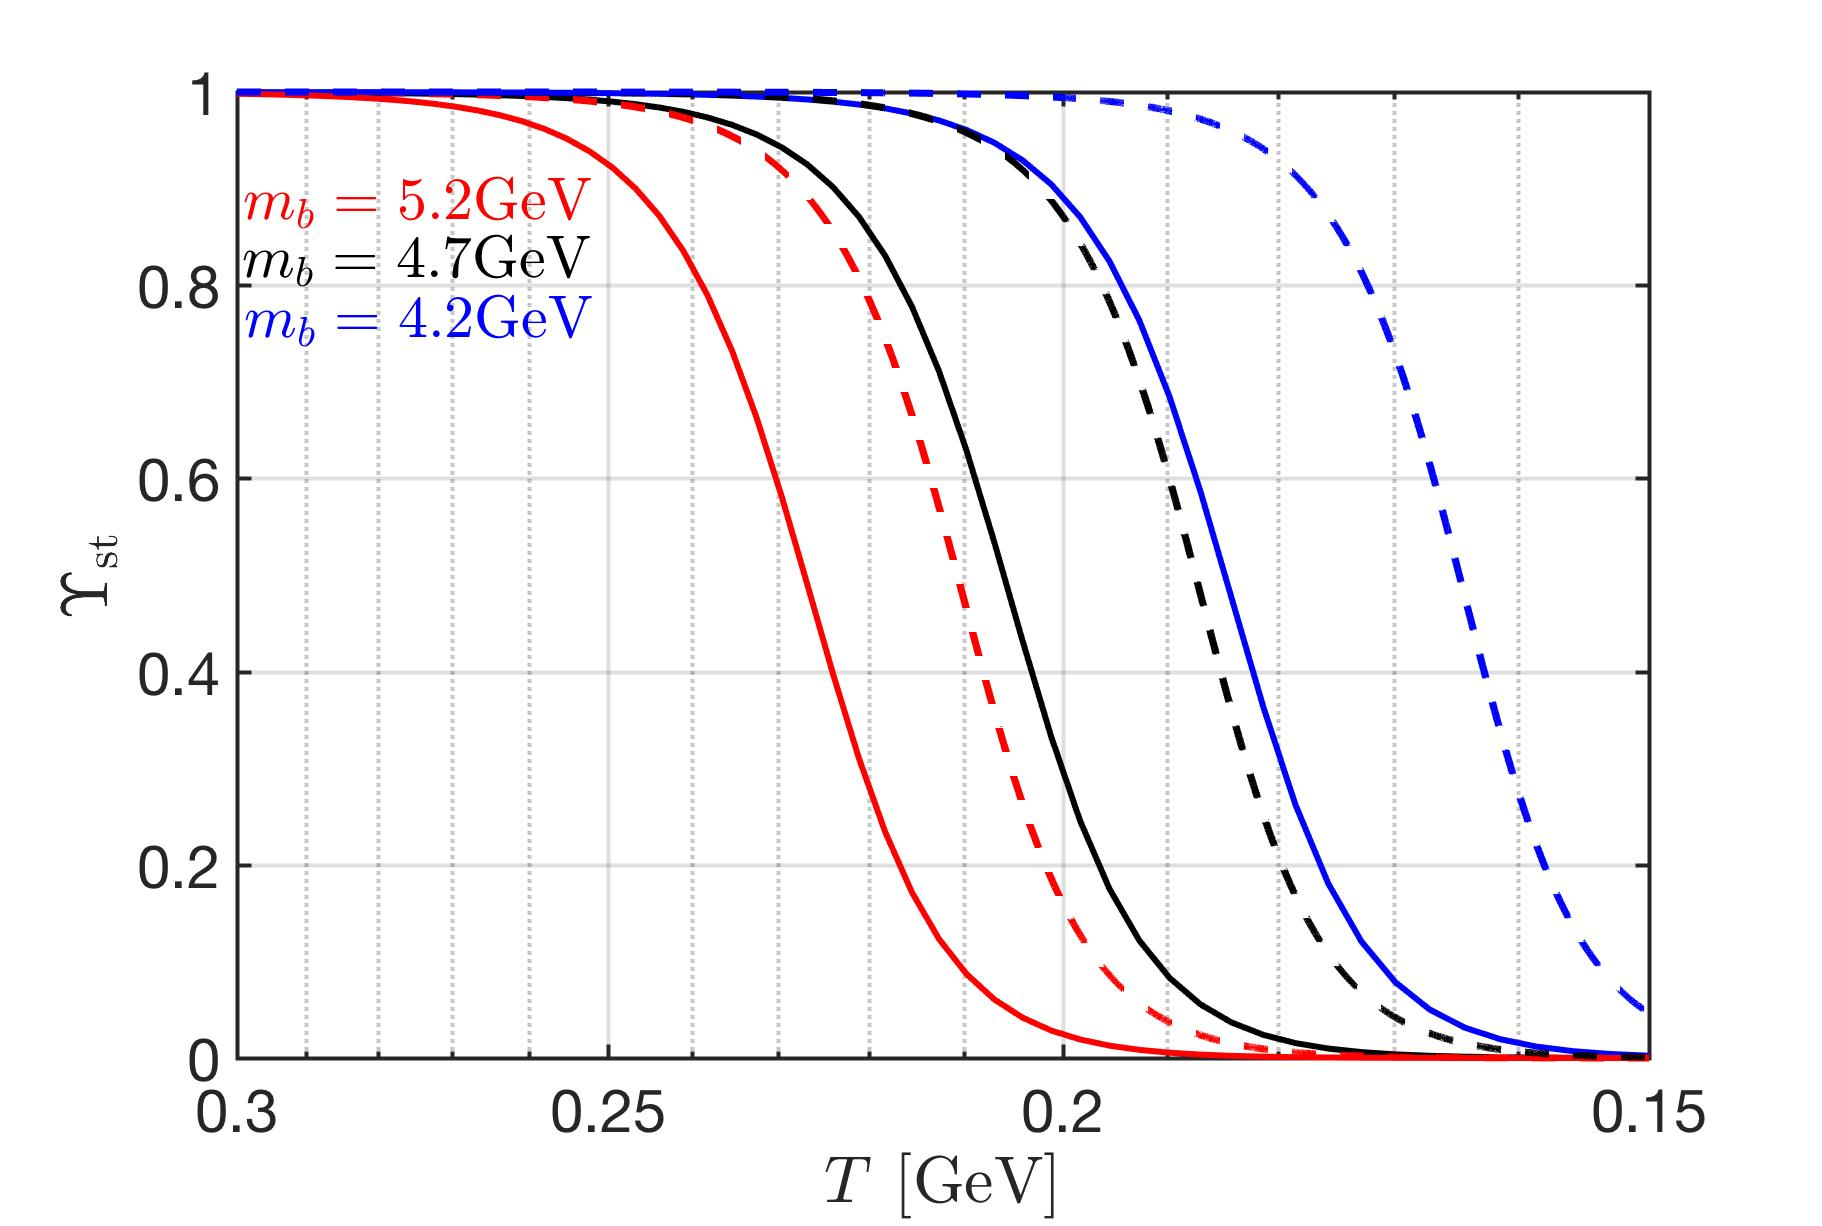
\includegraphics[width=\textwidth]{./plots/BquarkFugacity_tot}
\caption{\cccite{universe9070309}, adapted from thesis of C.T.Yang \cite{Yang:2024ret}.The fugacity of free/ bounded bottom quark as a function of temperature in the early Universe for $m_b=4.2\,\mathrm{GeV}$ (blue), $m_b=4.7\,\mathrm{GeV}$ (black), and $m_b=5.2\,\mathrm{GeV}$ (red). The solid lines represent the case bottom quark bound into $B_c$ mesons, and the dashed lines label the case of  free bottom quark.}
\label{fugacity_bc}
\end{center}
\end{figure}
%~~~~~~~~~~~~~~~~~~~~~~~~~~~~~~~~~~~~~~~~~~~~~~~~~~~~~~~~~~~~~~~~~~~~~~~~~~~~~~~~~~~~~~~~~~~~~~~
\,
In Fig.~\ref{fugacity_bc} the fugacity of bottom quark $\Upsilon_{\mathrm{st}}$ as a function of temperature, Eq.~(\ref{Fugacity_Sol}) is shown around the temperature $T=0.3\,\mathrm{GeV}>T>0.15\,\mathrm{GeV}$ for different masses of bottom quarks. In all cases we see prolonged non-equilibrium, this happens since the decay and reformation rates of bottom quarks are comparable to each other as we have noted in Fig.~\ref{ReactionTime} where both lines cross. One of the key results shown in Fig.~\ref{fugacity_bc} is that the smaller mass of bottom quark slows the strong interaction formation rate to the value of weak interaction decays just near the phase transformation of QGP to HG phase. Finally, the stationary fugacity corresponds to the reversible reactions in the stationary Universe. In this case, there is no arrow in time for bottom quark because of the detailed balance.



\subsubsection{Non-stationary correction in expanding Universe}

The Universe is expanding and temperature is a function of time. In this section we now consider the fugacity as a function of time and study the correction in fugacity due to the expanding Universe. In general, the fugacity of bottom quark can be written as 
\begin{align}\label{Nonstationary_sol}
&\Upsilon_b=\Upsilon_{\mathrm{st}}+\Upsilon^{\mathrm{non}}_{\mathrm{st}}=\Upsilon_\mathrm{st}\left(1+x\right),\quad x\equiv{\Upsilon_\mathrm{st}^{\mathrm{non}}}/{\Upsilon_\mathrm{st}},
\end{align}
where the variable $x$ corresponds to the correction due to non-stationary Universe. Substituting the general solution Eq.(\ref{Nonstationary_sol}) into differential equation Eq.(\ref{Fugacity_Eq0}), we obtain
\begin{align}\label{Nonstationary_eq}
\frac{dx}{dt}=-x^2\frac{\Upsilon_\mathrm{st}}{\tau_{source}}&-x\left[\frac{1}{\tau_{eff}}+3H-\frac{1}{\tau_T}\right]-\left[\frac{d\ln\Upsilon_\mathrm{st}}{dt}+3H-\frac{1}{\tau_T}\right],
\end{align}
where the effective relaxation time $1/\tau_{eff}$ is defined as
\begin{align}
\frac{1}{\tau_{eff}}\equiv\left[\frac{2\Upsilon_\mathrm{st}}{\tau_{source}}+\frac{1}{\tau_{decay}}+\frac{d\ln\Upsilon_\mathrm{st}}{dt}\right].
\end{align}
%~~~~~~~Figure~~~~~~~~~~~~~~~~~~~~~~~~~~~~~~~~~~~~~~~~~~~~~~~~~~~~~~~~~~~~~~~~~~~~~~~~~~~~~~~~~
\begin{figure}[t]
\begin{center}
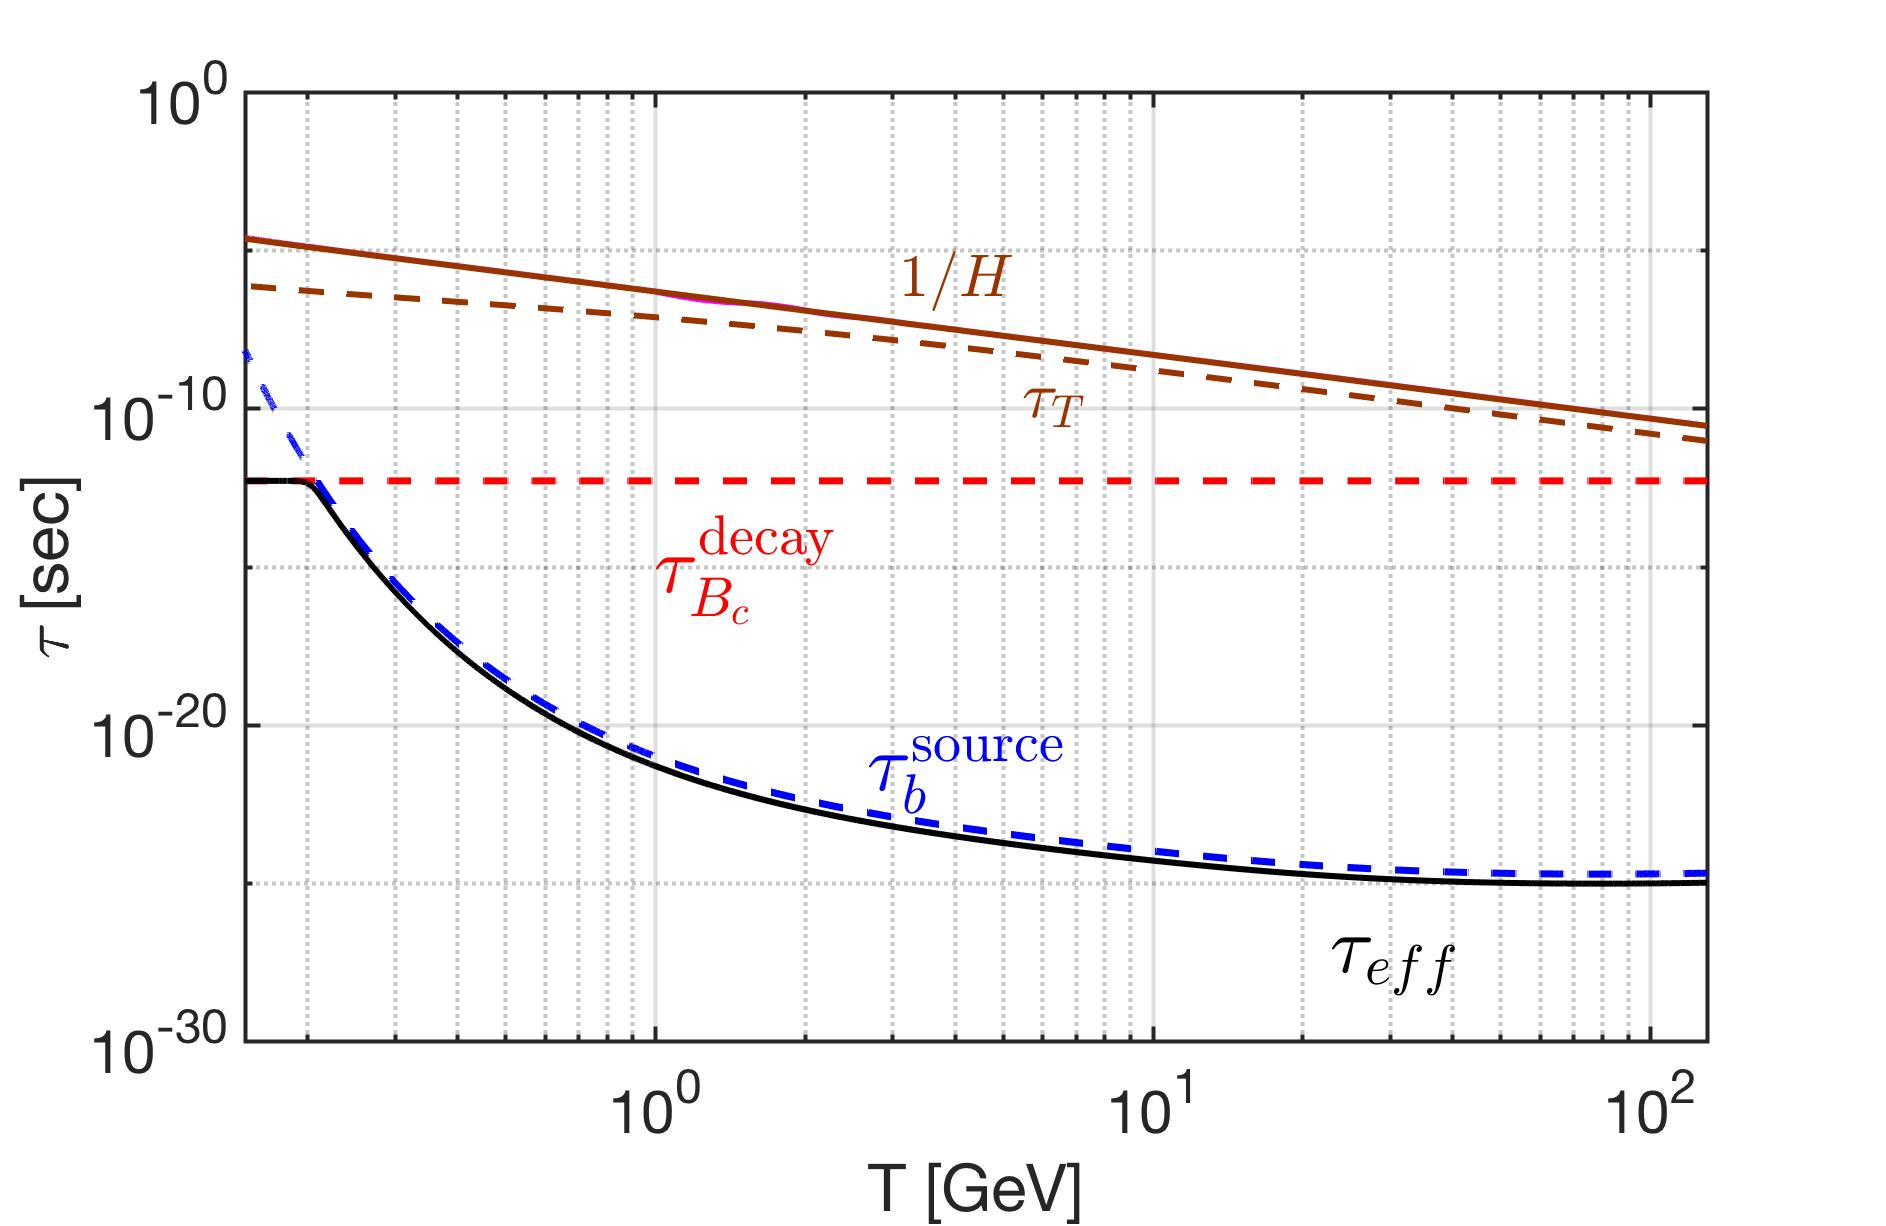
\includegraphics[width=\textwidth]{./plots/Tau_RelaxationTime002}
\caption{The effective relaxation time $\tau_{eff}$ as a function of temperature in the early Universe for bottom mass $m_b=4.7$GeV.  For comparison, we also plot the vacuum lifespan of $B_c$ meson $\tau_{B_c}^{decay}$(red dashed-line), the relaxation time for bottom production $\tau^b_{source}$ (blue dashed-line), Hubble expansion time $1/H$(brown solid line) and relaxation time for temperature cooling $\tau_T$(brown dashed-line). Adapted from thesis of C.T.Yang \cite{Yang:2024ret}.}
\label{RelaxationTime_eff}
\end{center}
\end{figure}
%~~~~~~~~~~~~~~~~~~~~~~~~~~~~~~~~~~~~~~~~~~~~~~~~~~~~~~~~~~~~~~~~~~~~~~~~~~~~~~~~~~~~~~~~~~~~~~~
In Fig.~\ref{RelaxationTime_eff} we see that when temperature is near to $T=0.2$ GeV, we have $1/\tau_{eff}\approx10^{7}H$, and $1/\tau_{eff}\approx10^5/\tau_T$. In this case, the last two terms in Eq.~(\ref{Nonstationary_eq}) compare to $1/\tau_{eff}$ can be neglected, and the differential equation becomes
\begin{align}\label{nonstationary_eq}
\frac{dx}{dt}=-\frac{x^2\,\Upsilon_\mathrm{st}}{\tau_{source}}&-\frac{x}{\tau_{eff}}-\left[\frac{d\ln\Upsilon_\mathrm{st}}{dt}+3H-\frac{1}{\tau_T}\right],
\end{align}


To solve the variable $x$ we consider the case $dx/dt,x^2\ll1$ first, we neglect the terms $dx/dt$ and $x^2$ in Eq.~(\ref{nonstationary_eq})  then solve the linear fugacity equation.  We will establish that these approximations are justified by checking the magnitude of the solution. Neglecting terms $dx/dt$ and $x^2$ in Eq.~(\ref{nonstationary_eq}) we obtain
\begin{align}
x\approx\tau_{eff}\left[\frac{d\ln\Upsilon_\mathrm{st}}{dt}+3H-\frac{1}{\tau_T}\right].
\end{align}
It is convenient to change the variable from time to temperature. For an isentropically-expanding universe, we have
\begin{align}\label{tau_H}
\frac{dt}{dT}=-\frac{\tau^\ast_H}{T},\qquad \tau^\ast_H=\frac{1}{H}\left(1+\frac{T}{3g^s_\ast}\frac{dg^s_\ast}{dT}\right).
\end{align}
In this case, we have
\begin{align}
x=\tau_{eff}\left[\frac{1}{\Upsilon_\mathrm{st}}\frac{d\Upsilon_\mathrm{st}}{dT}\frac{T}{\tau^\ast_H}+3H-\frac{1}{\tau_T}\right].
\end{align}
Finally, we can obtain the nonstationary fugacity by multiplying the fugacity ratio $x$ with $\Upsilon_\mathrm{st}$, giving
\begin{align}
\Upsilon_{\mathrm{st}}^{\mathrm{non}}
&\approx\left(\frac{\tau_{eff}}{\tau^\ast_H}\right)\left[\frac{d\Upsilon_\mathrm{st}}{dT}T-\Upsilon_{\mathrm{st}}\left(3H\tau^\ast_H-\frac{\tau^\ast_H}{\tau_T}\right)\right].
\end{align}

In Fig.~\ref{NonFugacity} we plot the nonstationary $\Upsilon^{\mathrm{non}}_\mathrm{st}$ as a function of temperature. The nonstationary fugacity $\Upsilon^{\mathrm{non}}_\mathrm{st}$ follows the behavior of $d\Upsilon_{\mathrm{st}}/dT$, which corresponds to the irreversible process in expanding Universe. In this case, the irreversible nonequilibrium process creates the arrow in time for bottom quark in the Universe. The large value of Hubble time compares to the effective relaxation time suppressing the value of nonstationary fugacity to $\mathcal{O}\sim10^{-7}$, which shows that the neglecting $dx/dt,x^2\ll1$ is a good approximation for solving the non-stationary fugacity in the early Universe.
%~~~~~~~Figure7~~~~~~~~~~~~~~~~~~~~~~~~~~~~~~~~~~~~~~~~~~~~~~~~~~~~~~~~~~~~~~~~~~~~~~~~~~~~~~~~~
\begin{figure}[t]
\begin{center}
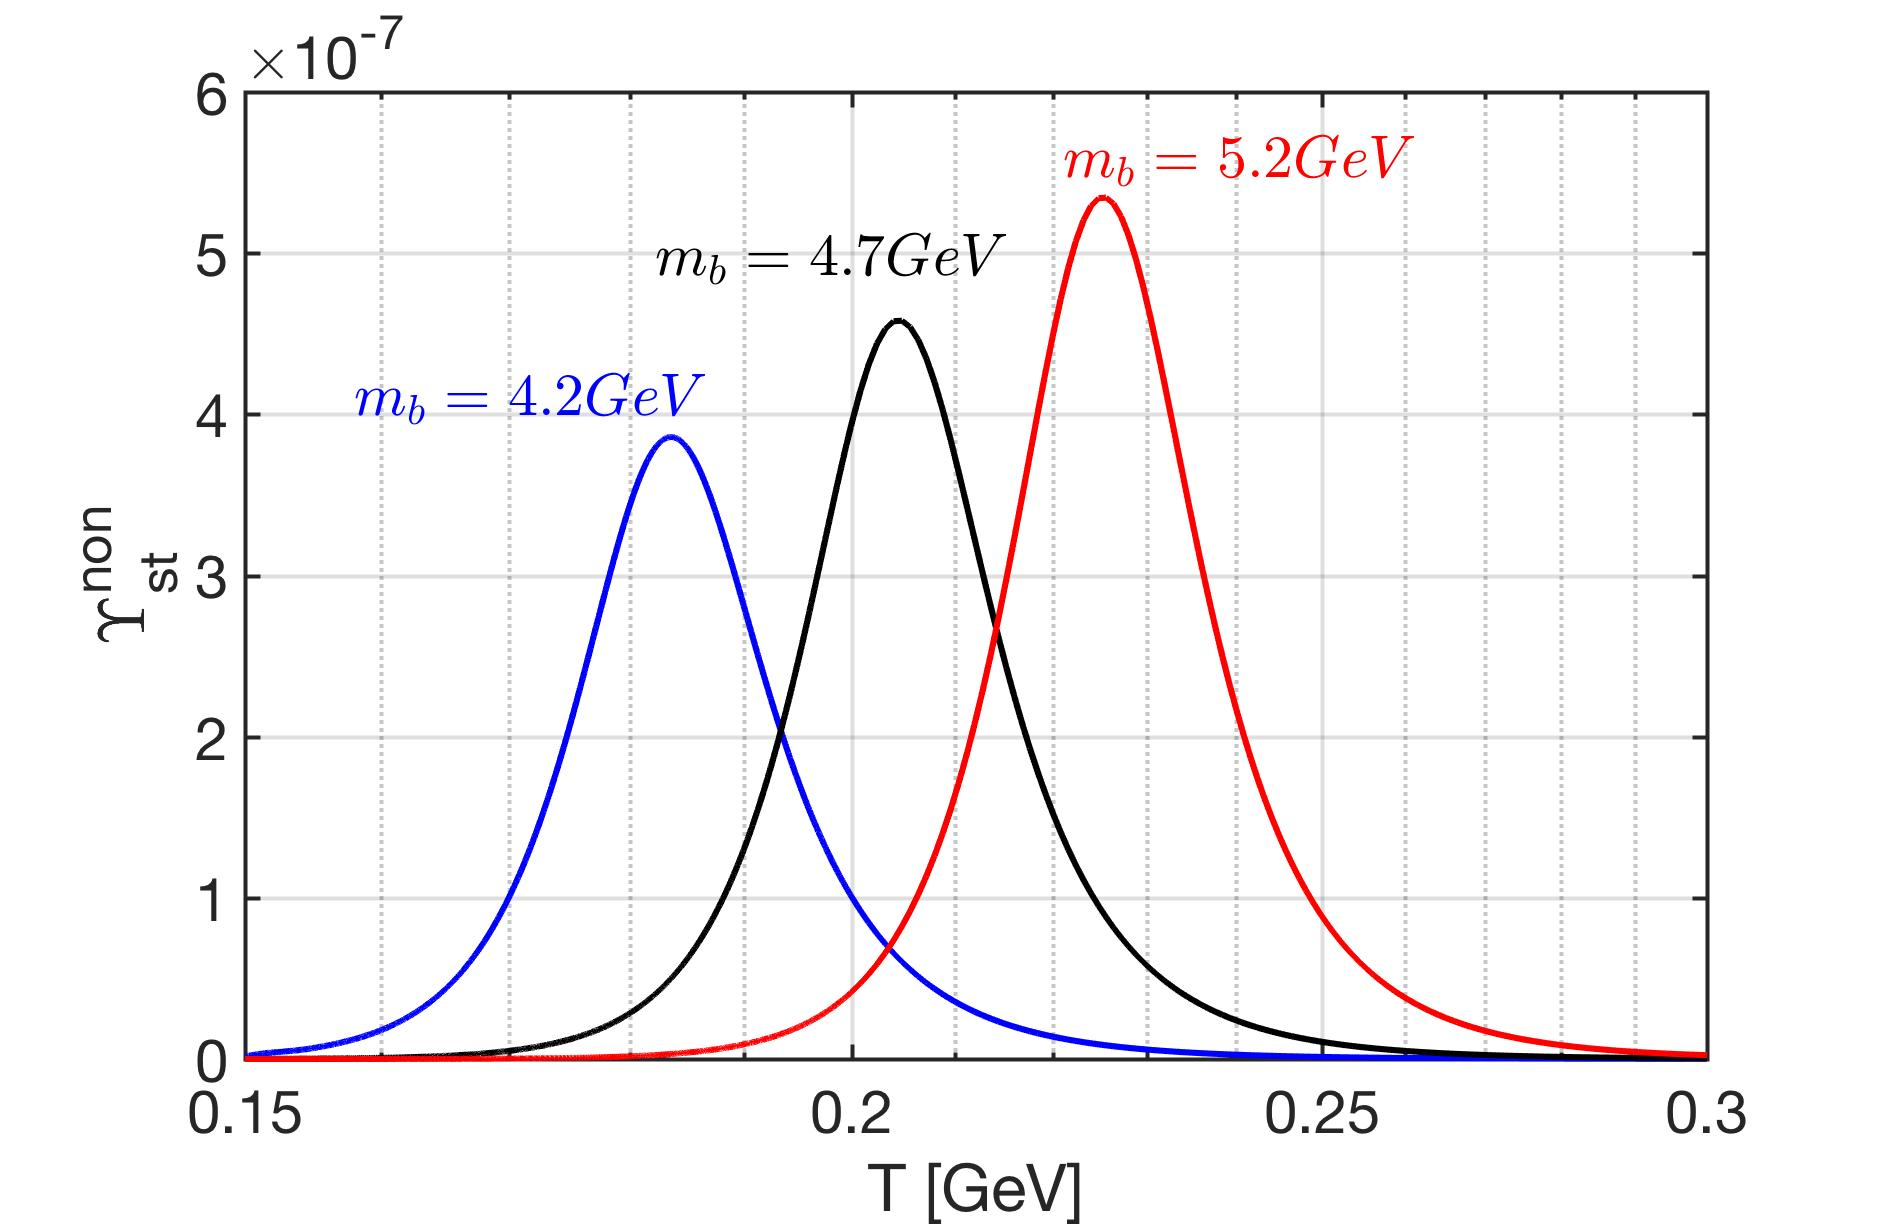
\includegraphics[width=\textwidth]{./plots/NonstationaryFugacity}
\caption{The non-stationary fugacity $\Upsilon_\mathrm{st}^{\mathrm{non}}$ as a function of temperature in the Universe for different bottom mass $m_b=4.2\,\mathrm{GeV}$ (blue), $m_b=4.7\,\mathrm{GeV}$ (black), and $m_b=5.2\,\mathrm{GeV}$ (red) for the case bottom  quarks bound into $B_c$ mesons. Adapted from thesis of C.T. Yang \cite{Yang:2024ret}.}
\label{NonFugacity}
\end{center}
\end{figure}
%~~~~~~~~~~~~~~~~~~~~~~~~~~~~~~~~~~~~~~~~~~~~~~~~~~~~~~~~~~~~~~~~~~~~~~~~~~~~~~~~~~~~~~~~~~~~~~~

To conclude this chapter, we have demonstrated that the bottom quark nonequliibrium occurs near the QGP phase transition around the temperature $T=0.3\sim0.15$ GeV in Fig.~\ref{fugacity_bc} and Fig.~\ref{NonFugacity}. We show the competition between weak interaction decay and the strong interaction $g+g\to b+\bar b$, $q+\bar q \to b+\bar b$ fusion processes drive the bottom quark departure from the equilibrium and create the arrow of time in the early Universe at relatively low QGP temperature. The results provide a strong motive for exploring the physics of baryon nonconservation involving the bottomnium mesons or/and bottom quarks in a thermal environment.

%~~~~~~~~~~~~~~~~~~~~~~~~~~~~~~~~~~~~~~~~~~~~~~~~~
%~~~~~~~~~~~~~~~~~~~~~~~~~~~~~~~~~~~~~~~~~~~~~~~~~
%{Introduction\daggerfootnote{This chapter has been published previously as \citet{Gottbrath1999}.}}

%\begin{figure}
%\centering
%\includegraphics[angle=0,width=\columnwidth]{fig1.pdf}
%\caption[]{}
%\label{fig1}
%\end{figure}